\documentclass{report}


\usepackage[T1]{fontenc}
\usepackage[utf8]{inputenc}
\usepackage{amsmath}


\usepackage{enumerate}
\usepackage{trfsigns}
\usepackage{graphicx}
\usepackage{fancyhdr}
\usepackage{lettrine}
\usepackage{hyperref}
\usepackage{subcaption}
\usepackage{tikz}
\usepackage{cite}
\usepackage{listings}
\usepackage[nottoc, numbib]{tocbibind}
\usepackage[ngerman]{babel}
\usepackage[Glenn]{fncychap}
\usepackage{trfsigns}
\usepackage{parskip}
\usepackage{microtype}


\usetikzlibrary{shapes}
\usetikzlibrary{arrows}
\usetikzlibrary{arrows.meta,topaths}
\usetikzlibrary{bending}
\usetikzlibrary{calc}
\title{Elektrotechnik 1 Praktikum 1}


\usepackage[
	includehead,
	headheight = 17mm,
	footskip = \dimexpr\headsep+\ht\strutbox\relax,
	tmargin = 0mm,
	bmargin = \dimexpr17mm+2\ht\strutbox\relax,
]{geometry}

\usepackage{anyfontsize}
\usepackage{float}
\usepackage{xcolor}

\definecolor{DarkGreenBlue}{HTML}{264653}
\definecolor{LightGreenBlue}{HTML}{2A9D8F}
\definecolor{LightOrange}{HTML}{E9C46A}
\definecolor{DarkOrange}{HTML}{F4A261}
\definecolor{RedOrange}{HTML}{E76F51}
\definecolor{BrightRed}{HTML}{D62828}
\definecolor{DeepBlue}{HTML}{003049}

\lstdefinestyle{code}{
	backgroundcolor=\color{backcolour},
	commentstyle=\color{codegreen},
	keywordstyle=\color{magenta},
	numberstyle=\tiny\color{codegray},
	stringstyle=\color{codepurple},
	basicstyle=\ttfamily\footnotesize,
	breakatwhitespace=false,
	breaklines=true,
	captionpos=b,
	keepspaces=true,
	numbers=left,
	numbersep=5pt,
	showspaces=false,
	showstringspaces=false,
	showtabs=false,
	tabsize=2
}

\definecolor{codegreen}{rgb}{0,0.6,0}
\definecolor{codegray}{rgb}{0.5,0.5,0.5}
\definecolor{codepurple}{rgb}{0.502,0.502,0.0}
\definecolor{backcolour}{rgb}{0.95,0.95,0.95}

\pagestyle{fancy}
\fancyhead[L]{\leftmark}
\fancyhead[R]{}
\fancyfoot[L]{}
\fancyfoot[C]{\thepage}
\fancyfoot[R]{\includegraphics[scale=0.2]{../assets/images/haw.jpg}}
\renewcommand\headrulewidth{0.5pt}


\begin{document}


\thispagestyle{empty}
\begin{tikzpicture}[overlay,remember picture]
	\thispagestyle{empty}
	\fill[black!2] (current page.south west) rectangle (current page.north east);

	\begin{scope}[transform canvas ={rotate around ={45:($(current page.north west)+(-.5,-6)$)}}]

		\shade[rounded corners=18pt, left color=DarkGreenBlue, right color=LightGreenBlue] ($(current page.north west)+(-.5,-6)$) rectangle ++(9,1.5);

	\end{scope}

	\begin{scope}[transform canvas ={rotate around ={45:($(current page.north west)+(.5,-10)$)}}]

		\shade[rounded corners=18pt, left color=LightOrange,right color=DarkOrange] ($(current page.north west)+(0.5,-10)$) rectangle ++(15,1.5);

	\end{scope}

	\begin{scope}[transform canvas ={rotate around ={45:($(current page.north west)+(0.5,-10)$)}}]

		\shade[rounded corners=8pt, right color=DarkOrange, left color=LightOrange] ($(current page.north west)+(1.5,-9.55)$) rectangle ++(7,.6);

	\end{scope}

	\begin{scope}[transform canvas ={rotate around ={45:($(current page.north)+(-1.5,-3)$)}}]

		\shade[rounded corners=12pt, left color=DeepBlue!80, right color=DeepBlue!60] ($(current page.north)+(-1.5,-3)$) rectangle ++(9,0.8);

	\end{scope}

	\begin{scope}[transform canvas ={rotate around ={45:($(current page.north)+(-3,-8)$)}}]

		\shade[rounded corners=28pt, left color=BrightRed, right color=BrightRed!80] ($(current page.north)+(-3,-8)$) rectangle ++(15,1.8);

	\end{scope}

	\begin{scope}[transform canvas ={rotate around ={45:($(current page.north west)+(4,-15.5)$)}}]

		\shade[rounded corners=25pt, left color=RedOrange, right color=DarkOrange] ($(current page.north west)+(4,-15.5)$) rectangle ++(30,1.8);

	\end{scope}

	\begin{scope}[transform canvas ={rotate around ={45:($(current page.north west)+(13,-10)$)}},]

		\shade[rounded corners=22pt, left color=DeepBlue,right color=DarkGreenBlue] ($(current page.north west)+(13,-10)$) rectangle ++(15,1.5);

	\end{scope}

	\begin{scope}[transform canvas ={rotate around ={45:($(current page.north west)+(18,-8)$)}},]

		\shade[rounded corners=8pt, left color=DarkOrange] ($(current page.north west)+(18,-8)$) rectangle ++(15,0.6);

	\end{scope}

	\begin{scope}[transform canvas ={rotate around ={45:($(current page.north west)+(19,-5.65)$)}},]

		\shade[rounded corners=12pt, left color=RedOrange] ($(current page.north west)+(19,-5.65)$) rectangle ++(15,0.8);

	\end{scope}

	\begin{scope}[transform canvas ={rotate around ={45:($(current page.north west)+(20,-9)$)}}]

		\shade[rounded corners=20pt, left color=BrightRed, right color=BrightRed!80] ($(current page.north west)+(20,-9)$) rectangle ++(14,1.2);

	\end{scope}

	\draw[ultra thick,gray] ($(current page.center)+(5,2)$) -- ++(0,-3cm) node[midway,left=0.25cm,text width=5cm,align=right,black!75]{{\fontsize{25}{30} \selectfont 
\includegraphics[width=\textwidth]{./assets/img/HAW_logo.png}}} node[midway,right=0.25cm,text width=6cm,align=left,orange]{{\fontsize{70}{86} \selectfont 2023}};

	\node at ($(current page.center)+(0,-4)$) {{\fontsize{40}{72} \selectfont Leistungselektronik}};

	\node[text width=8cm,align=center] at ($(current page.center)+(0,-6.5)$) {{\fontsize{16}{20} \selectfont \textcolor{orange}{ \bf \today}} \\[3pt] Steffen Reimers 2540209\\[3pt] PF: Emily Antosch 2519935 \\[3pt] Timo Türk 2545824\\[3pt]};

\end{tikzpicture}

\newpage

\tableofcontents

\listoffigures

\newpage
\chapter{Energietechnik - Praktikum 2 - Synchronmaschine}
\section{Einleitung}


In diesem Labor erfolgt die Analyse einer Drehstromsynchronmaschine (SM), die zu den am häufigsten verwendeten Maschinen in Kraftwerken gehört und zur Stromerzeugung eingesetzt wird. Die in diesem Experiment genutzte Maschine ist eine Außenpolmaschine mit vier Polen. Die Drehstromsynchronmaschine wird durch eine Gleichstrommaschine (GM) angetrieben, deren Erregung durch eine steuerbare Gleichstromquelle (Feldsteller) erfolgt.


\section{Kenndaten der Maschinen}

Dem Typenschild der Synchronmaschine wurden folgende Kenndaten entnommen:

\begin{itemize}
	\item Polpaare: 2
	\item $U_{N} = 380V$
	\item $I_{N} = 8A$
	\item $n_{N} = 1500min^{-1}$
\end{itemize}

Und für die Gleichstrommaschine:

\begin{itemize}
	\item $U_{N} = 400V$
	\item $I_{N} = 23,6A$
	\item $n_{N} = 1580min^{-1}/3000min^{-1}$
\end{itemize}


\subsection{Leerlaufversuch}

In diesem Teil des Versuchs wird die Leerlaufkennlinie, also die Funktion $U_{str} = f(I_{Err})$, aufgenommen. Dazu wird die Gleichstrommaschine auf die Nenndrehzahl $n_{N} = 1500min^{-1}$ gebracht, wobei Synchronmachine keine Erregung erfährt. Darauf hin wird der Erregerstrom langsam hoch gedreht und die entsprechende Leiter-Sternpunkt-Spannung $U_{str}$ wird aufgenommen. Es ist interessant zu sehen, dass selbst bei ausgeschalteter Erregung eine kleine Spannung im Läufer der Synchronmaschine zu messen ist. Das liegt an der Restmagnetisierung des Läufers, die durch die Drehbewegung eine Spannung induziert. Im Labor ist diese Spannung zwar sehr geringfügig, in großen Kraftwerken kann eine solche Spannung schon bereits gefährlich sein. Eine nicht erregte, aber bewegte Synchronmachine kann also schon gefährlich sein und unter Spannung stehen. Sobald die Frequenz der induzierten Spannung bei $50Hz$ angekommen ist, kann die Messung durchgeführt werden. Dabei sind die Werte aus Tabelle \ref{tab:leerlaufversuch} entstanden.

\begin{table}[!ht]
	\centering
	\begin{tabular}{llll}
		\hline
		$U_{str}$ in $V$ & $U_{N}$ in $V$ & $n$   & $I_{Err}$ in $A$ \\ \hline
		$2,9$            & $5,9$          & $0$   & $0$              \\
		$22,04$          & $38$           & $0,1$ & $0,075$          \\
		$43,82$          & $76$           & $0,2$ & $0,152$          \\
		$65,72$          & $114$          & $0,3$ & $0,232$          \\
		$87,51$          & $152$          & $0,4$ & $0,315$          \\
		$109,5$          & $190$          & $0,5$ & $0,398$          \\
		$131,7$          & $228$          & $0,6$ & $0,481$          \\
		$153,6$          & $266$          & $0,7$ & $0,565$          \\
		$175,3$          & $304$          & $0,8$ & $0,66$           \\
		$197,4$          & $342$          & $0,9$ & $0,773$          \\
		$219,6$          & $380$          & $1,0$ & $0,925$          \\
		$241$            & $418,3$        & $1,1$ & $1,21$           \\ \hline
	\end{tabular}
	\caption{Die Werte des Leerlaufversuchs}
	\label{tab:leerlaufversuch}
\end{table}

\subsection{Kurzschlussversuch}
Die obere Messreihe wird wiederholt. Allerdings werden nun die Klemmen der Synchronmaschine kurzgeschlossen und der Kurzschlussstrom wird gemessen und aufgetragen. Zusammen mit den Messungen aus dem Leerlaufversuch kann so das Ersatzschaltbild der Synchronmaschine ermittelt werden.
\begin{table}[!ht]
	\centering
	\begin{tabular}{lll}
		\hline
		$Ik$ in $A$ & $n$   & $IErr$ in $A$ \\ \hline
		$0$         & $0$   & $0,049$       \\
		$0,8$       & $0,1$ & $0,103$       \\
		$1,6$       & $0,2$ & $0,214$       \\
		$2,4$       & $0,3$ & $0,323$       \\
		$3,2$       & $0,4$ & $0,433$       \\
		$4,0$       & $0,5$ & $0,543$       \\
		$4,8$       & $0,6$ & $0,653$       \\
		$5,6$       & $0,7$ & $0,762$       \\
		$6,4$       & $0,8$ & $0,871$       \\
		$7,2$       & $0,9$ & $0,981$       \\
		$8,0$       & $1,0$ & $1,091$       \\
		$8,8$       & $1,1$ & $1,199$       \\ \hline
	\end{tabular}
	\caption{Die Werte des Kurzschlussversuchs}
	\label{tab:kurzschlussversuch}
\end{table}

\subsection{Polradspannung}
\label{sec:polradspannung}

Um die Polradspannung zu ermitteln, wird der Leerlaufversuch wieder aufgebaut. Nachdem die Synchronmaschine mittels der Gleichstrommaschine auf die Nenndrehzahl von $1500min^{-1}$ gebracht wurde, wird der Erregerstrom so eingestellt, dass sich beim Kurzschlussversuch $I_{k} = I_{N}$ einstellen würde (vgl. Tabelle \ref{tab:kurzschlussversuch}). Dann wird nun die Spannung zwischen den Klemmen $U$ und $V$ gemessen. Die Polradspannung ergibt sich dann zu $U_{PN} = 234V$.

\subsection{Kennlinien}
\label{sec:kennlinien}

Mit den vorher ermittelten Messwerten können nun die Graphen erstellt werden. Die Kennlinien der Synchronmachine sind durch Regression an die Messwerte angepasst worden.

\begin{figure}[!ht]
	\centering
	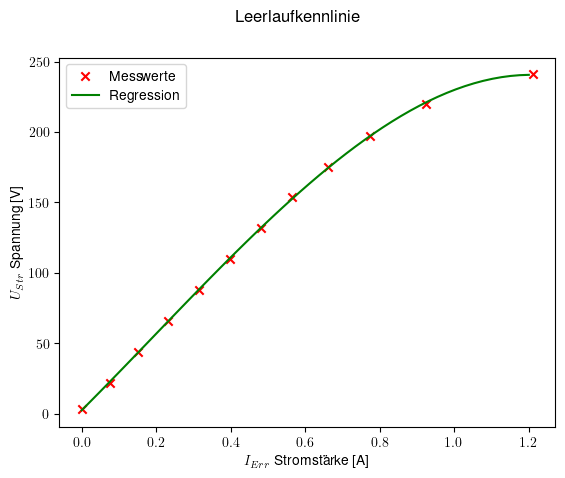
\includegraphics[width=0.9\textwidth]{./assets/img/leerlauf_kennlinie.png}
	\caption{Leerlaufkennlinie aus den Messwerten}
	\label{fig:leerlaufkennlinie}
\end{figure}

Die Leerlaufkennlinie (siehe \ref{fig:leerlaufkennlinie}) stellt den Verlauf der Leiter-Nullleiterspannung zum Erregerstrom dar. Es ist erkennbar, dass diese Kennlinie nicht ganz linear verläuft und gegen Ende der Kennlinie eher einen logarithmischen Verlauf annimmt. Die Regression wurde daher auch mit einer nicht-linearen, kubischen Gleichung vorgenommen. Für diesen Wertebereich sind die Messwerte aber dafür ziemlich genau geworden.

\begin{figure}[!ht]
	\centering
	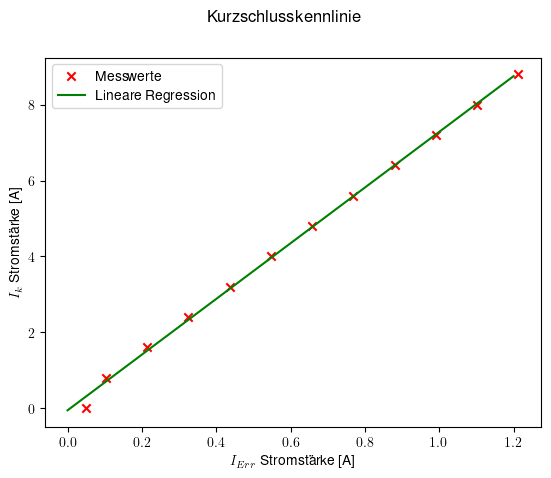
\includegraphics[width=0.9\textwidth]{./assets/img/kurzschluss_kennlinie.png}
	\caption{Kurzschlusskennlinie aus den Messwerten}
	\label{fig:kurzschlusskennlinie}
\end{figure}

Die Kurzschlusskennlinie (siehe \ref{fig:kurzschlusskennlinie}) stellt den Verlauf des Leiterstroms zum Erregerstrom dar. Diese ist, im Gegensatz zur Leerlaufkennlinie mithilfe von linearer Regression angenähert und ist vom Verlauf der Messpunkte her auch deutlich linearer. Auch auf diese Messpunkte passt die lineare Regression ziemlich genau.

Mithilfe dieser Werte kann nun das Kurzschlussverhältnis im Leerlauf ermittelt werden:

\begin{equation}
	\label{eq:1}
	K_{C} = \frac{I_{Err, L}}{I_{Err,k}} = \frac{0,925A}{1,09A} = 0,849
\end{equation}

Für die Reaktanz $X_{d}$ wird die Strangspannung aus der Kennlinie abgelesen ($\frac{380V}{\sqrt{3}} = 219,39V$). Der Kurzschlussstrom bei dem entsprechenden Erregerstrom ($0,912$) wird dann von der Kennlinie des Kurzschlussstroms abgelesen. Es ergibt sich:

\begin{equation}
	\label{eq:2}
	X_{d} = \frac{U_{N,Str}}{I_{k}} = \frac{219,39V}{6,63A} = 33,09\Omega
\end{equation}

Zum Schluss wird dann noch aus der Strangspannung $U_{N,Str}$ und dem Nennstrom $I_{N}$ die Nennimpedanz $Z_{N}$ der Synchronmachine bestimmt:

\begin{equation}
	\label{eq:3}
	Z_{N} = \frac{U_{N,Str}}{I_{N}} = \frac{219,39V}{8A} = 27,42\Omega
\end{equation}


\section{Inselbetrieb}
\label{sec:inselbetrieb}


Im Inselbetrieb ist die Synchronmaschine nicht mit dem Versorgungsnetz verbunden. Stattdessen fungiert sie als Generator, der die angeschlossenen Verbraucher mit elektrischer Energie versorgt. Im Experiment wird die Synchronmaschine mithilfe der Gleichstrommaschine auf ihre Nenndrehzahl (1500 min^−1) gebracht und anschließend durch ohmsche oder induktive Lasten belastet.

\subsection{Ohmsche Verbraucher}
\label{sec:ohmsche-verbraucher}

In dem ersten Versuch zum Inselbetrieb werden rein-ohmsche Verbraucher an die Synchronmachine angeschlossen. Dazu wird ein Lastwiderstand im Stern an die Klemmen der Synchronmaschine verschaltet. Der Lastwiderstand kann dann über einen Mechanismus verstellt werden. Die Last ist dabei immer symmetrisch. Wichtig dabei zu bedenken, ist es, die Belastungsgrenzen der Synchronmachine im Auge zu behalten. Um einer Beschädigung der Anlage vorzubeugen ist hier also Vorsicht geboten. Begonnen wird mit dem höchstmöglichen Widerstand.

\begin{table}[!ht]
	\centering
	\begin{tabular}{llllllll}
		\hline
		$R [\Omega]$ & $U_{str} [V]$ & $U_{N} [V]$ & $I_{str} [A]$ & $I_{N} [A]$ & $P [kW]$ & $Q [var]$ & $S [kVA]$ \\ \hline
		$76$         & $219,4$       & $380$       & $2,74$        & $2,74$      & $1,804$  & $104,2$   & $1,806$   \\
		$63,9$       & $219,9$       & $380,9$     & $3,3$         & $3,3$       & $2,173$  & $119$     & $2,176$   \\
		$54,6$       & $219,3$       & $379,8$     & $3,8$         & $3,8$       & $2,617$  & $158,6$   & $2,521$   \\
		$47,5$       & $219,9$       & $380,8$     & $4,4$         & $4,4$       & $2,898$  & $187$     & $2,903$   \\
		$42,4$       & $219,6$       & $380,3$     & $4,9$         & $4,9$       & $3,24$   & $200$     & $3,250$   \\
		$37,8$       & $219,6$       & $380,4$     & $5,52$        & $5,52$      & $3,62$   & $233$     & $3,634$   \\
		$34,3$       & $219,5$       & $380,1$     & $6,1$         & $6,1$       & $4,009$  & $243$     & $4,015$   \\
		$31,6$       & $219,7$       & $380,3$     & $6,7$         & $6,7$       & $4,375$  & $272$     & $4,38$    \\
		$29,1$       & $219,8$       & $380,4$     & $7,24$        & $7,24$      & $4,743$  & $275$     & $4,731$   \\ \hline
	\end{tabular}
	\label{tab:ohm_messreihe_1}
\end{table}

Nach einem Widerstandswert von $29,1\Omega$ wurde die Messreihe abgebrochen, da die Leistungs- und Stromwerte schon sehr nah an der Grenze für den Betrieb der Synchronmachine waren.

In der zweiten Messreihe wird der Erregerstrom konstant auf einen Wert von $I_{Err} = 1,1A$ gehalten. Daher können auch alle Widerstandswerte aufgenommen werden. Die aufgenommenen Werte der Messung sind in Tabelle \ref{tab:ohm_messreihe_2} aufgeführt.
\begin{table}[!ht]
	\centering
	\begin{tabular}{llllllll}
		\hline
		$R [\Omega]$ & $U_{str} [V]$ & $U_{N} [V]$ & $I_{str} [A]$ & $I_{N} [A]$ & $P [kW]$ & $Q [var]$ & $S [kVA]$ \\ \hline
		$76$         & $221$         & $382,8$     & $2,76$        & $2,76$      & $1,831$  & $106,7$   & $1,834$   \\
		$63,9$       & $217$         & $376,6$     & $3,27$        & $3,27$      & $2,123$  & $126,6$   & $2,127$   \\
		$54,6$       & $213$         & $368$       & $3,7$         & $3,7$       & $2,374$  & $150,1$   & $2,378$   \\
		$47,5$       & $207,8$       & $359,7$     & $4,16$        & $4,16$      & $2,585$  & $166,7$   & $2,59$    \\
		$42,4$       & $202$         & $350,6$     & $4,55$        & $4,55$      & $2,75$   & $171$     & $2,76$    \\
		$37,8$       & $195,8$       & $339,2$     & $4,92$        & $4,92$      & $2,881$  & $186$     & $2,886$   \\
		$34,3$       & $188$         & $326$       & $5,2$         & $5,2$       & $2,946$  & $184$     & $2,952$   \\
		$31,6$       & $182$         & $315$       & $5,5$         & $5,5$       & $3,012$  & $187$     & $3,017$   \\
		$29,1$       & $175$         & $303$       & $5,7$         & $5,7$       & $3,038$  & $173$     & $3,042$   \\
		$27,3$       & $169$         & $293$       & $5,9$         & $5,9$       & $3,031$  & $169$     & $3,035$   \\
		$25,4$       & $160$         & $278$       & $6,1$         & $6,1$       & $2,981$  & $150$     & $2,987$   \\
		$23,5$       & $153$         & $268$       & $6,29$        & $6,29$      & $2,94$   & $145$     & $2,943$   \\
		$22,6$       & $150$         & $260$       & $6,4$         & $6,4$       & $2,9$    & $140$     & $2,902$   \\
		$21,1$       & $143$         & $248$       & $6,5$         & $6,5$       & $2,83$   & $133$     & $2,832$   \\
		$20,1$       & $137$         & $240$       & $6,67$        & $6,67$      & $2,776$  & $132,4$   & $2,778$   \\
		$19,0$       & $131$         & $230$       & $6,77$        & $6,77$      & $2,704$  & $129,5$   & $2,707$   \\ \hline
	\end{tabular}
	\label{tab:ohm_messreihe_2}
	\caption{Die Messreihe für $I_{Err} = 1,1A$ und rein-ohmscher Verbraucher}
\end{table}

Es ist deutlich zu erkennen, dass bei dieser Messreihe die Leistung mit sinkenden Widerstandswert zunächst steigt, bei $29,1\Omega$ ihren Höhepunkt hat und dann ab dem Punkt wieder sinkt. Mit dieser Messung lässt sich nun auch ein Zeigerdiagramm zeichnen. Da es sich hier um einen rein-ohmschen Verbraucher handelt, stehen die Strangspannung ($U_{str}$) und die Spannung über die Reaktanz ($U_{Xd}$) rechtwinklig aufeinander.

\begin{figure}[!ht]
	\centering
	\includegraphics[width=0.9\textwidth]{./assets/img/Inselbetrieb378IE.png}
	\caption{Der zeitliche Verlauf von Strom und Spannung bei $I_{Err} = 1,1A$ und rein-ohmschen Verbraucher bei $R=37,8\Omega$}
	\label{fig:inselbetrieb_ohm_oszi}
\end{figure}

Aus den Werten aus dem Tabelle bei Widerstand $29,1\Omega$, also $P=3,083kW$, $I_{N} = 5,7A$ und $U_{str} = 175V$, und den Werten, die in \ref{eq:2} und \ref{eq:3} berechnet wurden, lassen sich nun die Werte für das Zeigerdiagramm bestimmen. Da wir einen rein-ohmschen Verbraucher haben gilt $\phi = 0°$.

\begin{equation}
	\label{eq:4}
	U_{Xd} = X_{d} \cdot I_{N} = 33,09\Omega \cdot 5,7A = 188,613V
\end{equation}

Für $U_{P}$ folgt:

\begin{equation}
	\label{eq:5}
	U_{P} = \sqrt{U_{Xd}^{2} + U_{str}^{2}} = \sqrt{(188,613V)^{2} + (175V)^{2}} = 257,293V
\end{equation}

\begin{equation}
	\label{eq:6}
	\theta = arctan(\frac{U_{Xd}}{U_{str}}) = arctan(\frac{188,613V}{175V}) = 47,144°
\end{equation}

\subsection{Induktive Last}
\label{sec:induktive-last}

Zusätzlich zu der Betrachtung eines rein-ohmschen Verbrauchers soll nun auch ein rein induktiver Verbraucher analysiert werden. Dazu stehen im Labor auch Lastinduktivitäten bereit, die auch wieder im Stern verschaltet werden.


\begin{table}[!ht]
	\centering
	\begin{tabular}{llllllll}
		\hline
		$L [mH]$ & $U_{str} [V]$ & $U_{N} [V]$ & $I_{str} [A]$ & $I_{N} [A]$ & $P [W]$ & $Q [kvar]$ & $S [kVA]$ \\ \hline
		$360$    & $219$         & $379,5$     & $1,7$         & $1,7$       & $93,7$  & $1150$     & $1154$    \\
		$220$    & $219$         & $379,8$     & $2,9$         & $2,9$       & $153$   & $1896$     & $1902$    \\ \hline
	\end{tabular}
	\label{tab:induk_messreihe_1}
	\caption{Messreihe für den rein induktiven Verbraucher bei $U_{N} = U = konst.$}
\end{table}

Aufgrund der Belastungsgrenzen der Maschine und von zeitlichen Einschränkungen wurde die Messung der induktiven Last bei konstanter Spannung $U_{N}$ auf zwei Messpunkte beschränkt. Es ist zu erkennen, dass die Messreihe in Tabelle \ref{tab:induk_messreihe_1} analog zu der in Tabelle \ref{tab:ohm_messreihe_1} ist. Allerdings ist natürlich jetzt hauptsächlich Blindleistung zu messen, die durch die Induktivitäten verbraucht wird.


\begin{table}[!ht]
	\centering
	\begin{tabular}{llllllll}
		\hline
		$L$   & $Ustr$ & $UN$  & $Istr$ & $IN$   & $P$     & $Q$    & $S$    \\ \hline
		$360$ & $210$  & $364$ & $1,6$  & $1,6$  & $86,4$  & $1060$ & $1063$ \\
		$220$ & $192$  & $332$ & $2,55$ & $2,55$ & $118,5$ & $1455$ & $1459$ \\
		$114$ & $153$  & $265$ & $3,92$ & $3,92$ & $151$   & $1787$ & $1792$ \\
		$42$  & $83$   & $145$ & $5,8$  & $5,8$  & $143$   & $1459$ & $1465$ \\ \hline
	\end{tabular}
	\label{tab:induk_messreihe_2}
	\caption{Messreihe für den rein induktiven Verbraucher bei $I_{Err} = 1,1A$}
\end{table}

Für die zweite Messreihe ergibt sich, wie auch schon im ersten Versuch zum Inselbetrieb (vgl. Tabelle \ref{tab:ohm_messreihe_2}), dass bei $L=114mH$ die Blindleistung und Scheinleistung der Schaltung am höchsten ist. Für alle anderen Werte für die Induktivitäten ergibt sich ein niedrigerer Wert.

\begin{figure}[!ht]
	\centering
	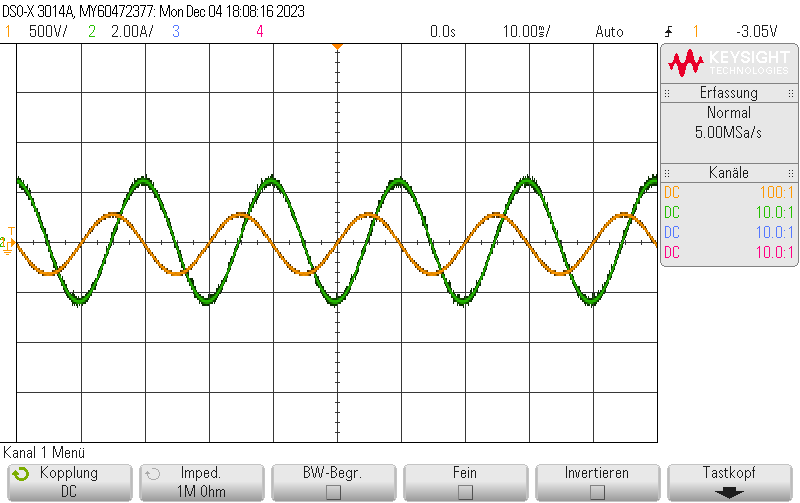
\includegraphics[width=0.9\textwidth]{./assets/img/Inselbetrieb360mHIE1.1.png}
	\caption{Der zeitliche Verlauf der Spannung und des Stroms beim Inselbetrieb und rein-induktiver Last}
	\label{fig:insel_reininduk_oszi}
\end{figure}

Mithilfe der Messung aus Tabelle \ref{tab:induk_messreihe_2} kann nun erneut das Zeigerdiagram erstellt werden. Dazu werden der Tabelle an der Stelle $L=360mH$ die Werte $P=86,4W$, $I_{N} = 1,6A$ und $U_{str} = 210V$ entnommen. Für $U_{Xd}$ gilt dann:

\begin{equation}
	\label{eq:7}
	U_{Xd} = X_{d} \cdot I_{N} = 33,09\Omega \cdot 1,6A = 52,944V
\end{equation}

Da es sich hier in der Versuchsreihe um eine rein-induktive Last handelt, ist der Winkel zwischen der Strangspannung $U_{str}$ und der Spannung über der Reaktanz $U_{Xd}$ $0°$. Die beiden Spannungen stehen also aufeinander und die Spannung $U_{P}$ kann durch Vektoraddition ermittelt werden:

\begin{equation}
	\label{eq:8}
	U_{P} = U_{str} + U_{Xd} = 210V + 52,944V = 262,944V
\end{equation}


\section{Synchronisation mit dem Netz}
\label{sec:synchr-mit-dem}

In diesem Versuchsteil wird die Synchronmaschine mit den Versorgungsnetz gekoppelt.

\subsection{Synchronisation auf das starre Netz}
\label{sec:synchr-auf-das}

Um einen Generator mit dem starren Synchronisation zu synchronisieren, müssen die folgenden vier Vorraussetzungen erfüllt sein:

\begin{itemize}
	\item Die Spannungshöhe von Einpeisung und Netz müssen gleich sein
	\item Die Frequenz von Einspeisespannung und Netzspannung müssen übereinstimmen
	\item Die Phasenlage der Phasen der Einspeisung müssen gleich sein mit den Phasen des Netzes
	\item Die Drehfeldrichtung des Generators müssen mit dem Drehfeld des Netzes passen.
\end{itemize}

Sollte einer dieser Punkte nicht erfüllt sein, kann es beim Synchronisieren im schlechtesten Fall einen elektrischen Kurzschluss geben. Um das zu verhindern, können mithilfe einer Dunkelschaltung (vgl. Abbildung \ref{fig:dunkelschaltung_aufbai}) die Übereinstimmung zwischen Netz und Einspeisung überprüft werden. Diese besteht einfach zwei Leuchtmittel pro Phase, die in Reihe geschaltet sind. Es sind zwei Leuchtmittel, da im schlechtesten Fall bei der Synchronisation $2\cdot \hat{u} = 2\cdot 325V = 650V$ auf einer Phase liegen. Da es sich um baugleiche Leuchtmittel handelt, wird die Spannung auf beide Leuchtmittel gleichmäßig aufgeteilt und es kommt nicht zu einer Überbelastung der Lampen.

\begin{figure}[!ht]
	\centering
	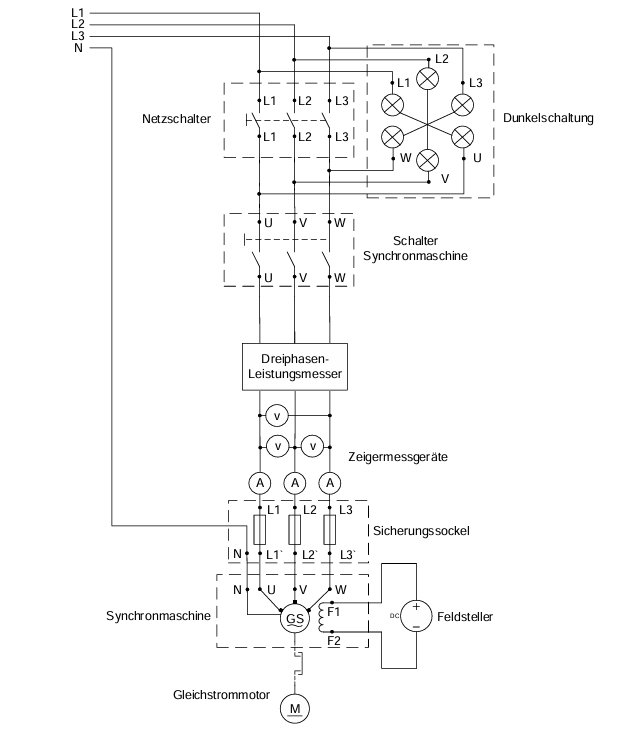
\includegraphics[width=0.9\textwidth]{./assets/img/dunkelschaltung_aufbau.png}
	\caption{Aufbau der Synchronisationsschaltung als Dunkelschaltung}
	\label{fig:dunkelschaltung_aufbau}
\end{figure}

Das Funktionsprinzip dieser Schaltung beruht darauf, dass die Lampen beim erfolgreichen Zeitpunkt der Synchronisation erlöschen. Dies geschieht, weil zu diesem Zeitpunkt auf beiden Seiten der Dunkelschaltung dasselbe Potenzial vorhanden ist und somit kein Strom fließt. Trotz ihrer Fehleranfälligkeit ermöglicht dieses Hilfsmittel eine einfache Beobachtung und Abstimmung der Kriterien. Ein Oszilloskop kann auch verwendet werden und kann auch ein sehr hilfreiches Werkzeug sein. Jedoch kann das Oszilloskop die Drehrichtung nicht unterscheiden, weshalb es in Kombination mit der Dunkelschaltung verwendet wird. Wenn sich die Drehrichtungen unterscheiden, zeigt die Dunkelschaltung ein rotierendes Lauflicht, bei dem immer ein Lampenpaar leuchtet, während die anderen beiden dunkel bleiben.

Neben der Dunkelschaltung kann auch eine Hellschaltung dafür verwendet werden, um den Punkt der Synchronisation zu bestimmen. Allerdings ist hier das Problem, dass der Punkt der maximalen Helligkeit deutlich schwerer festzustellen ist als der Punkt, an dem die Leuchten aus sind. Die Lampen bei der Hellschaltung sind fast gleich ausgebaut, wobei die Lampen nicht mehr hintereinander auf der gleichen Phase verschaltet sind sondern auf verschiedenen Phasen liegen. So ist die Phase L1 nicht mehr mit U verbunden sondern mit V.
Auch die Dunkelschaltung ist nicht perfekt. Da die Leuchtmittel eine Mindestspannung zum Leuchten benötigen, schaltet die Dunkelschaltung schon ein wenig vor dem optimalen Synchronisationspunkt ab und schalten sich auch erst ein wenig danach wieder an. Eine zweite Instanz zum Überprüfen der vier Kriterien ist in diesem Fall auch sinnvoll. Außerdem können automatische Einrichtungen verwendet werden, die den optimalen Synchronisationspunkt feststellen und dann den Generator auf das Netz schalten.

\subsection{Generatorbetrieb}
\label{sec:generatorbetrieb}

In diesem Laborteil wurde die auf das Netz geschaltete Synchronmaschine im generatorischen Betrieb untersucht, wobei sowohl der normalerregte als auch der übererregte Zustand berücksichtigt wurde. Die Experimente wurden mithilfe von Oszillographen dokumentiert. Um den generatorischen Betrieb zu realisieren, wurde die Frequenz der Strangspannung am Generator auf 50,1 Hz erhöht. Dies wurde durch Anheben der Spannung der Synchronmaschine erreicht, was zu einem größeren Drehmoment auf der Welle führte. Da die Netzfrequenz führend ist, ändert sich die Frequenz der Strangspannung nicht. Dennoch operiert die Synchronmaschine nun im generatorischen Betrieb. Die Messungen wurden sowohl aus Netzsicht als auch aus Maschinensicht durchgeführt. Diese Perspektiven unterscheiden sich in der Definition der Leistungsaufnahme oder -abgabe. Die Netzsicht betrachtet die Leistungsaufnahme des Netzes, während die Maschinensicht die Leistungsaufnahme der Maschine in Betracht zieht.

Alle folgenden Abbildung sind im Verbraucherzählsystem aufgenommen, da eine Änderung des Zählpfeilsystems lediglich eine Änderung der Betrachtungsweise ist.

\begin{figure}[!ht]
	\centering
	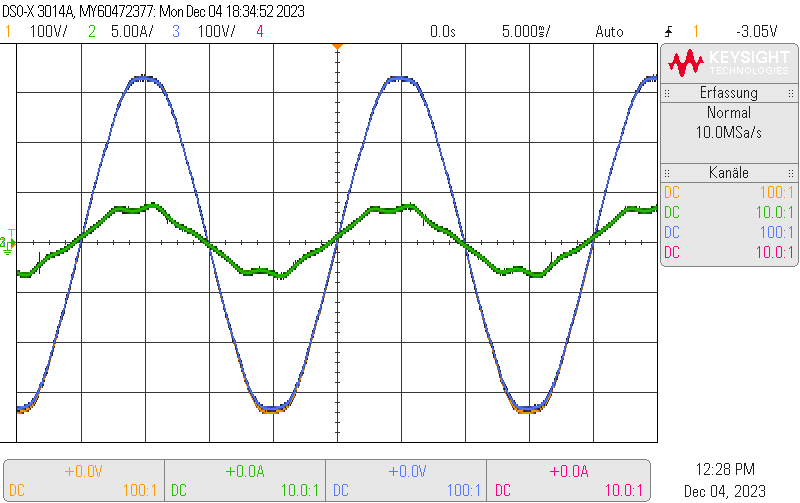
\includegraphics[width=0.9\textwidth]{./assets/img/synchronisation_netz_generator_ne_vzp.png}
	\caption{Oszillograph des Betriebs als Generator, Netzsicht und normalerregt}
	\label{fig:sngn}
\end{figure}

Die Abbildung \ref{fig:sngn} zeigt Strom und Spannung auf der Netzseite im normalerregten, generatorischen Zustand. Strom und Spannung liegen fast perfekt in Phase und das Netz nimmt annährend reine Wirkleistung auf. Das Netz verhält sich wie ein rein-ohmscher Verbraucher.

\begin{figure}[!ht]
	\centering
	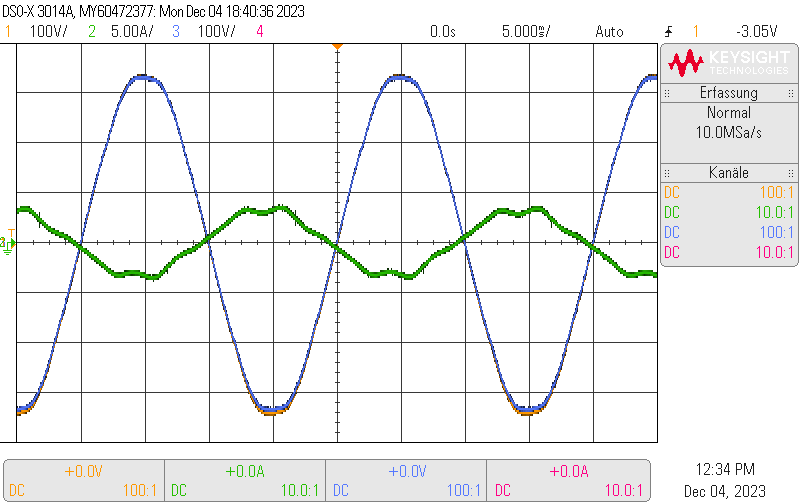
\includegraphics[width=0.9\textwidth]{./assets/img/synchronisation_maschine_generator_ne_vzp.png}
	\caption{Oszillograph des Betriebs als Generator, Maschinensicht und normalerregt}
	\label{fig:smgn}
\end{figure}

In Abbildung \ref{fig:smgn} ist der Strom und die Spannung auf der Maschinenseite im normalerregten, generatorischen Zustand zu sehen. Strom und Spannung liegen fast perfekt phasenverschoben um $180°$ vor. Das Produkt aus Strom und Spannung ist negativ, im Verbraucherzählsystem entspricht dies einer Abgabe von fast reiner Wirkleistung an das Netz.

\begin{figure}[!ht]
	\centering
	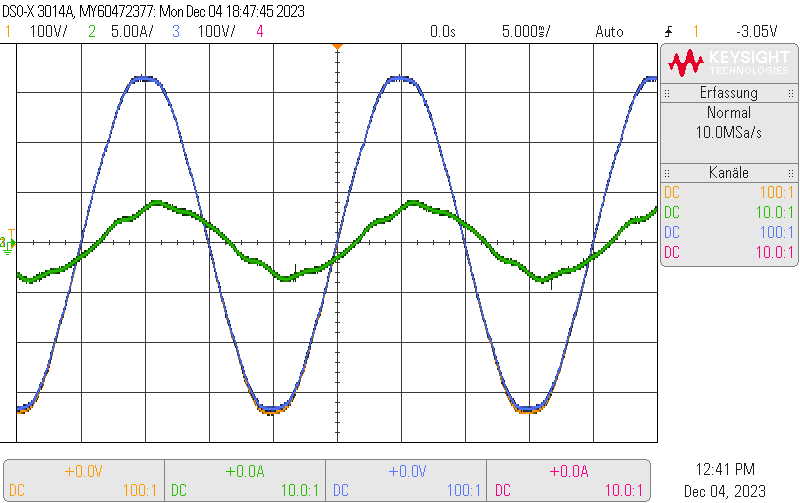
\includegraphics[width=0.9\textwidth]{./assets/img/synchronisation_netz_generator_uee_vzp.png}
	\caption{Oszillograph des Betriebs als Generator, Netzsicht und übererregt}
	\label{fig:sngue}
\end{figure}

In der nächsten Abbildung \ref{fig:sngue} ist der Verlauf von Strom und Spannung auf der Netzseite im übererregten, generatorischen Betrieb erkennbar. Der Strom eilt der Spannung ein wenig nach. Das Netz nimmt hier also nicht nur Wirkleistung, sondern auch induktive Blindleistung auf.

\begin{figure}[!ht]
	\centering
	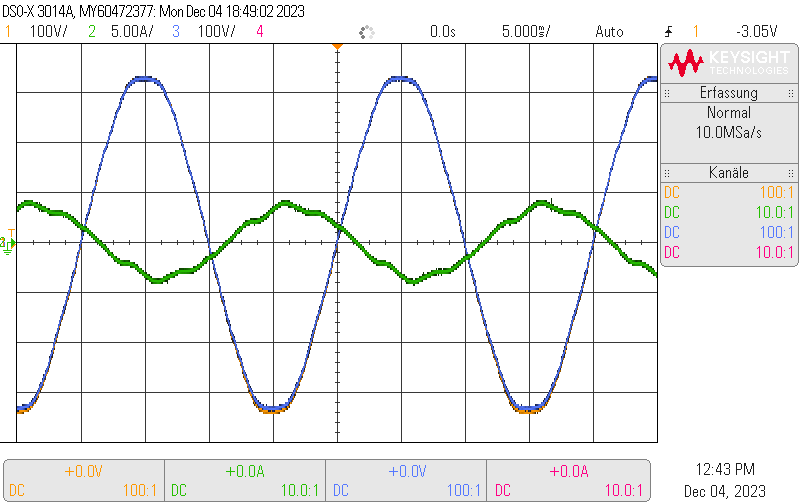
\includegraphics[width=0.9\textwidth]{./assets/img/synchronisation_maschine_generator_uee_vzp.png}
	\caption{Oszillograph des Betriebs als Generator, Maschinensicht und übererregt}
	\label{fig:smgue}
\end{figure}

Die Abbildung \ref{fig:smgue} zeigt Strom und Spannung auf der Maschinenseite im übererregten Zustand im Generatorbetrieb. Das Produkt aus Strom und Spannung ist hier wieder negativ. Der Strom eilt der Spannung ein wenig vor. Die Maschine gibt also Wirk- und induktive Blindleistung ab. Man könnte auch sagen, dass die Maschine kapazitive Blindleistung aus dem Netz aufnimmt.

\begin{figure}[!ht]
	\centering
	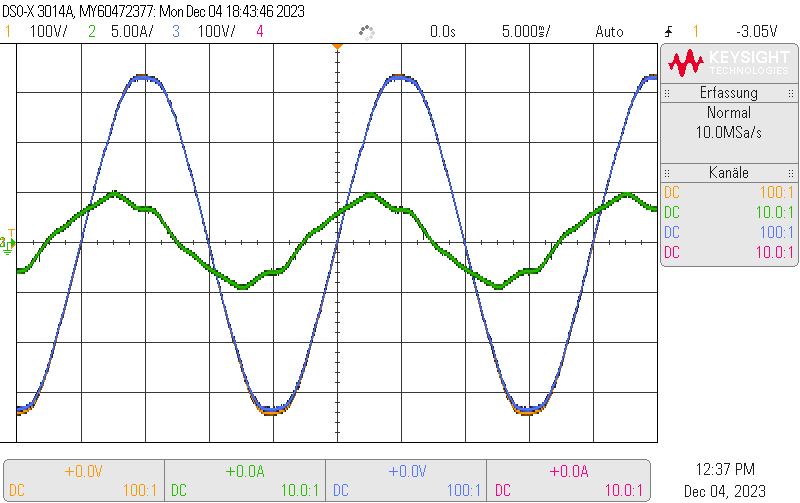
\includegraphics[width=0.9\textwidth]{./assets/img/synchronisation_netz_generator_ue_vzp.png}
	\caption{Oszillograph des Betriebs als Generator, Netzsicht und untererregt}
	\label{fig:sngu}
\end{figure}

In der nächsten Abbildung \ref{fig:sngu} ist der Verlauf von Strom und Spannung auf der Netzseite im untererregten, generatorischen Betrieb erkennbar. Der Strom eilt der Spannung ein wenig vorraus. Das Netz nimmt hier also nicht nur Wirkleistung, sondern auch kapazitive Blindleistung auf.

\begin{figure}[!ht]
	\centering
	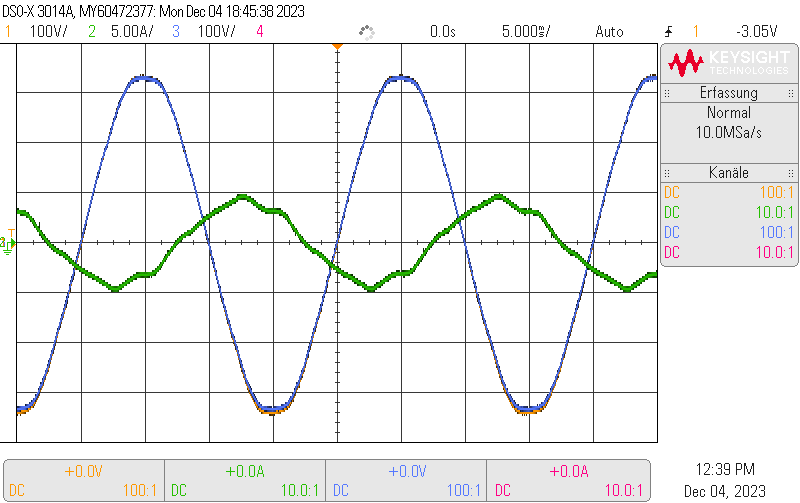
\includegraphics[width=0.9\textwidth]{./assets/img/synchronisation_maschine_generator_ue_vzp.png}
	\caption{Oszillograph des Betriebs als Generator, Maschinensicht und untererregt}
	\label{fig:smgu}
\end{figure}

In der letzten Abbildung \ref{fig:smgu} ist der Verlauf von Strom und Spannung auf der Maschinenseite im untererregten, generatorischen Betrieb zu sehen. Der Strom eilt der Spannung ein wenig nach und das Produkt aus Strom und Spannung sit negativ. Die Maschine gibt hier also sowohl Wirk- als auch kapazitive Blindleistung ab.

\subsection{Motorbetrieb}
\label{sec:motorbetrieb}

Für den Motorbetrieb wird die Frequenz, die durch die Gleichstrommaschine eingestellt wird, auf ca. $49,9Hz$ eingestellt. Da die Frequenz der Spannung vom Netz vorgegeben wird, führt eine Verringerung der Frequenz an der Maschine lediglich dazu, dass die Synchronmachine nun im Motorbetrieb läuft.

Aus Zeitgründen und dem geringen Mehrwert der Messungen wurden diese nicht mit Bildern begleitet.
\end{document}
